\subsection{Introduccion} 
Se esta diseñando un software de arquitectura, para el cual es necesario que dado un conjunto de edificios representados como rectangulos apoyados sobre una base en comun, se devuelva el perfil definido en el horizonte.\\
Estos edificios vienen representados por tuplas de tres elementos que representan donde comienza el edificio, su altura y donde termina, de las cuales tenemos que ir tomando en cada momento donde comienza un edificio la altura maxima alcanzada en ese punto.

 \subsection{Ejemplos y Soluciones}
 Consideremos el siguiente ejemplo del problema:\\
 $ [<3,2,5>;<1,4,2>;<4,1,6>;<6,8,10>]$ \\
  Cada una de estas tuplas de tres elementos se indica donde comienza el edificio en la primera coordenada, su altura en la segunda y donde termina en la tercera coordenada.\\
  
  Lo primero que hacemos es ordenar estas tuplas en orden creciente por lo que representa donde comienza el edificio (llamemosla pared izquierda), quedandonos de la siguiente manera:\\ 
$[<1,4,2>;<3,2,5>;<4,1,6>;<6,8,10>$] \\

Por otro lado ordenamos los edificios por la coordenada donde terminan (llamemosla pared derecha).\\
$[<1,4,2>;<3,2,5>;<4,1,6>;<6,8,10>$] \\

\subsection{Desarrollo}
Como mencionamos anteriormente, tenemos como datos de entrada la posici\'on donde comienza y termina cada edificio y adem\'as su altura, con lo cual representaremos a los edificios con tuplas de 3 elementos (posici\'on de inicio o pared izquierda, altura, y posici\'on donde termina o pared derecha). Primero organizaremos a los edificios en dos arreglos, donde cada arreglo contendr\'a el total de edificios, uno con un orden ascendente seg\'un pared izquierda y el otro tambi\'en con un orden ascendente pero seg\'un pared derecha. Adem\'as tendremos un conjunto en el que iremos agregando los edificios que ``comience'' y quitando los edificios que ``terminen'', es decir, aqu\'i� estar\'an los edificios ``activos'' (que ``empezaron'' y no ``terminaron'') en cada momento.
La idea del algoritmo es ir recorriendo las posiciones (del eje x) en las que haya una o m\'as paredes. En cada punto lo que haremos es agregar a mi conjunto de activos los edificios que en ese punto tengan su pared izquierda, o sea que est\'an "comenzando", y quitar a los edificios que all\'i tengan su pared derecha, o sea que est\'an ``terminando''. Una vez completada esta labor, buscaremos el edificio activo que tenga la altura m\'axima y nos lo guardaremos, llam\'emoslo Max. Se puede ver claramente que el borde superior de la silueta en un punto dado va a estar determinado por el edificio m\'as alto que haya en ese punto, es decir, el edificio activo m\'as alto. Como en cada paso podemos conseguir el edificio activo m\'as alto, proseguiremos as\'i� hasta el \'ultimo punto y habremos arm\'andonos la silueta.

\subsection{Demostraci\'on}
Demostraremos por inducci\'on que en cada paso de este algoritmo obtenemos la altura del edificio m\'as alto en ese punto.

P(i) =``Nuestro edificio Max es el edificio m\'as alto en el punto i''\\

Caso base, P(1):\\
En este caso nos encontramos con nuestro primer conjunto de paredes, que puede tener una o m\'as paredes. Este s\'olo puede tener paredes izquierda ya que es donde ``comienzan'' nuestros primeros edificios y ning\'un edificio ha empezado antes como para que aparezca una pared derecha indicando su ``finalizaci\'on''. Por lo tanto tenemos un conjunto de edificios que ``comienza'' en este punto y nos basta recorrer ese conjunto para encontrar el edificio de mayor altura, al cual llamaremos Max. Entonces, sin duda, Max es el edificio m\'as alto en este punto.

Paso inductivo, P(n) $\rightarrow$ P(n+1):
Nuestra hipótesis inductiva nos dice que el edificio más alto en el punto n es Max. Ahora veamos qué ocurre en n+1. En este punto podemos encontrar un conjunto que contiene tanto paredes izquierda como derecha, con lo cual separaremos a este conjunto de paredes en dos subconjuntos. Por un lado el conjunto de paredes izquierda, y por otro el de paredes derecha. Recorreremos primero el conjunto de paredes izquierda agregando cada edificio de este conjunto al conjunto de edificios activos. Cada vez que alguno supere a nuestro Max actual, ese será el nuevo Max. Si después terminar el recorrido nuestro Max anterior cambió, entonces ese nuevo Max será el edificio más alto en este punto (y no es posible que este nuevo Max tenga su pared derecha en este punto ya que eso implicaría que ese edificio está "empezando" y "terminando" en el mismo punto, lo cual no es válido). Y caso contrario seguiremos manteniendo nuestro Max de antes y deberemos fijarnos las paredes derecha para ver si este Max "termina".
Ahora recorreremos el conjunto de paredes derecha quitando cada edificio que aparezca en este conjunto de nuestro conjunto de activos y fijándonos si está "terminando" el edificio Max en cada paso. Entonces cada vez que aparezca una pared derecha del edificio Max actual, lo reemplazaré por el edificio activo más alto. Por lo tanto, después de terminar el recorrido, nuestro edificio Max es el más alto de los edificios en ese punto.

Teniendo las alturas máximas para cada punto, es trivial armarnos la silueta ya que con las alturas máximas ya tenemos su borde superior en cada punto.


\subsection{Complejidad}

definimos edificio = < izq :natural x alto : natural x der : natural >
definimos edificioenCero al que tiene todos sus elementos en cero.
\begin{algorithm}
\begin{algorithmic}[1]\parskip=1mm
 \caption{LaSilueta( ciudad: arreglo(edificios) , cantidadEdificios : natural)}
	
	\STATE{arregloXIzq \leftarrow ordenarXIzquierda(ciudad)}\\
	\STATE{arregloXDer \leftarrow ordenarXDerecha(ciudad)}\\
	\STATE{EdificiosActivos \leftarrow Multiconjunto(edificio)}\\
	\\
	\STATE{posIzquierdo , posDerecho \leftarrow 0}\\
	\STATE{max \leftarrow edificioenCero \\
	\STATE{mientras posIzquierdo < cantidadEdificios \&\& posDerecho < cantidadEdificios }\\
	\STATE{ \quad SI arregloXIzq.indice(posIquierdo).izq \leq arregloXDer.indice(posDerecho).der}\\
			\STATE{\quad\quad auxiliar \leftarrow arregloXIzq.indice(posIzquierdo)}\\
			\STATE{\quad\quad mientras auxiliar.izq = arregloXIzq.indice(posIquierdo).izq \&\& posIzquierdo != cantidadEdificios}\\
			\STATE{\quad\quad\quad agregar(arregloXIzq.indice(posIquierdo), EdificiosActivos )}\\
			\STATE{\quad\quad\quad SI arregloXIzq.indice(posIquierdo).alto > max.alto}\\
			\STATE{\quad\quad\quad\quad max \leftarrow arregloXIzq.indice(posIquierdo) }\\
		\STATE{\quad SI NO }\\
			\STATE{\quad\quad auxiliar \leftarrow arregloXDer.indice(posDerecha)}\\
			\STATE{\quad\quad mientras auxiliar.der = arregloXDer.indice(posDerecha).der && posDerecha != cantidadEdificios}\\
			\STATE{\quad\quad\quad SI  arregloXDer.indice(posDerecha).id = max.id}\\
			\STATE{\quad\quad\quad\quad dameMaximoSiguiente( arregloXDer.indice(posDerecha), EdificiosActivos)}\\
			\STATE{{\quad\quad\quad\quad sacar( arregloXDer.indice(posDerecha), EdificiosActivos)}
\\
\end{algorithmic}
Los algoritmos ordenarXizquierda y ordenarXDerecha es el conocido algoritmo mergeSort sacado del libro de brassard, la complejidad del mismo es \Ode{N*Log(N)} siendo N la cantidad de elementos en el arreglo, �sea todos los edificios, estos algoritmos ordenan los arreglos de tuplas, uno por la coordenada izq y el otro por la coordenada derecha respectivamente.\\
El multiconjunto EdificiosActivos esta representado con la estructura Multiset de la librer�a STL de c++, la relaci\'on de orden sobre los elementos que se defini\'o es por la coordenada alt y en el caso que la altura sea igual por la componente der.\\
Para las operaciones para agregar, sacar elementos la complejidad es \Ode{log(n)} siendo n la cantidad de elementos en el multiconjunto y para obtener el proximo maximo lo que se realiza es obtener la referencia al elemento que 
representa el m\'aximo, esto lleva \Ode{Log(n)} y luego se obtiene el posterior, en caso de no ser posible obtenemos el anterior, en el peor caso se tienen todos los edificios y la complejidad seria \Ode{log(N)}.\\
El ciclo de las lineas 9-12 se realiza para cada punto x donde haya paredes izquierdas, con lo cual la complejidad total sera la suma de todas las paredes izquierda, siendo esta N la cantidad de edificios. De la misma manera el ciclo de las lineas 15 a 18 se ejecuta para todas las paredes derechas de los edificios con lo cual el total de las iteraciones sera la suma de las paredes derechas �sea N. Como el ciclo principal se ejecuta mientras la cantidad de paredes recorridas izquierdas sea menor a la cantidad de edificios y la cantidad de paredes derechas sea menor a la cantidad de edificios y las iteraciones internas modifican las paredes izquierdas y derechas recorridas, el total de las iteraciones es 2*N, siendo N la cantidad total de edificios, con lo cual como la complejidad de agregar , sacar y obtener el m\'aximo es \Ode{log(N)} en el peor caso, el total es \Ode{2*N*Log(N)} $\subset$ \Ode{N*Log(N)} siendo esta la complejidad total del algoritmo y esta estrictamente menor a \Ode{N^2} como se solicitaba en el enunciado.

\end{algorithm}	
\newpage
\subsection{Experimentaci\'on}
Se realizaron experimentaciones sobre varios tipos de caso para observar el comportamiento del algoritmo, en todos los casos se generaron 1000 entradas, a las gr�ficas resultantes se las comparo con la funci�n n*log(n)*1000, siendo n la cantidad de edificios de entrada.\\
Para la primer ejecuci�n se realizo un an\'alisis sobre el algoritmo en edificios donde la distancia entre sus paredes izquierda y derecha era corta, estas se encontraban entre las posiciones 1 y 30, pero sus alturas variaban en el orden entre 1 y 10000, dando el siguiente gr�fico como resultado.\\
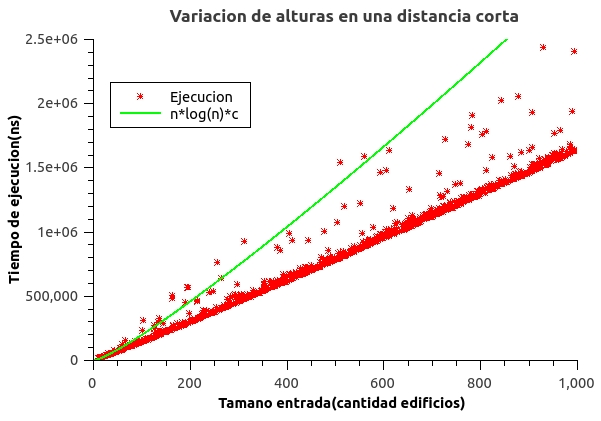
\includegraphics[scale=0.7]{Ej2/VariacionAlturas.jpg}
\\
El segundo gr\'afico corresponde a instancias generadas de manera random donde la altura se encontraba entre 1 y 40, pero las distancias entre la primer y la segunda pared de cada edificio varia entre los 1 y 2000 , elegido de manera random la posici�n de ambos lados pero siempre que sea entrada valida, \'osea el valor de la pared izquierda es mayor estricta a la de la pared derecha.
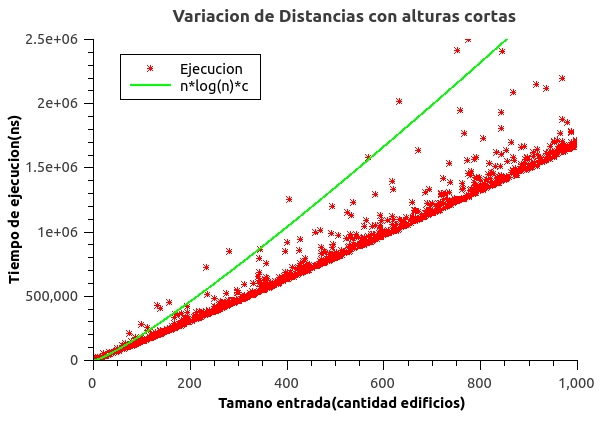
\includegraphics[scale=0.7]{Ej2/VariacionDistancias.jpg}
\\
Luego para el tercer gr\'afico consideramos que era importante ver como se comportaba el multiconjunto cuando se agregaban todos los edificios de la entrada, de esta manera se generaron entradas donde los edificios eran todos iguales, as\'i se ingresaban todos al multiconjunto y ve\'iamos como se comportaba el algoritmo, obteniendo este gr\'afico como resultado donde se ve que su complejidad es del orden logar\'itmico en la cantidad de edificios de entrada por la cantidad edificios.
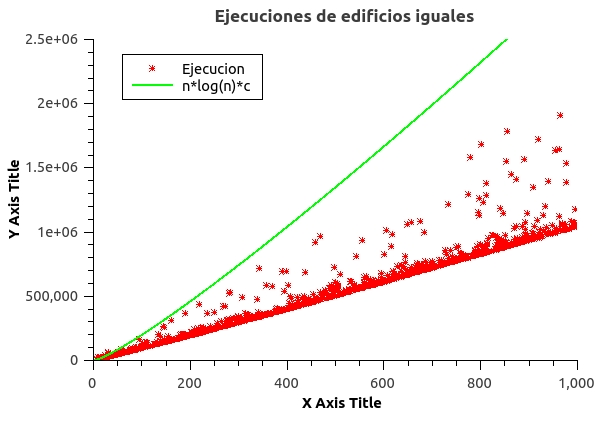
\includegraphics[scale=0.7]{Ej2/iguales.jpg}
\\
Por ultimo realizamos un gr�fico con entradas random donde las mismas variaban combinando todas las anteriores, obteniendo de nuevo que el orden era logar�tmico al compararlo con la funci�n.
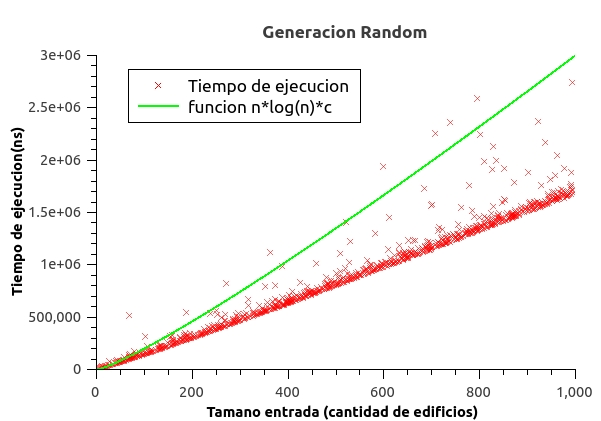
\includegraphics[scale=0.7]{Ej2/Random.jpg}
\\
 Concluimos por lo tanto que el algoritmo respeta los ordenes de complejidad ya que el or



